\section{Bayes'schen Netze}

Ein Bayes'schen Netz ist ein Graph, in dem Zufallsvariablen die Knoten und die bedingten Wahrscheinlichkeiten zwischen den Variablen die Kanten sind.

\paragraph{Aufabau eines Bayes'schen Netzes}

\begin{enumerate}
    \item Um ein Bayes'sches Netz aufzubauen, m�ssen zun�chst alle Zufallsvariablen und ihre Wertebereiche f�r eine bestimmte Anwendung identifiziert werden.
    \item Alle Zufallsvariablen werden in einem Netzwerk so angeordnet, dass alle Klauselabh�ngigkeiten zwischen Variablen durch Kanten dargestellt werden.
    \item F�r Variablen, die nicht voneinander abh�ngig sind, soll eine a priori Wahrscheinlichkeitsverteilung bestimmt werden.
\end{enumerate}

Wenn eine Variable \(Y\) direkt von den Variablen \(X_1\) bis \(X_n\) abh�ngt, m�ssen die bedingten Wahrscheinlichkeiten f�r alle Werte von \(i\) bestimmt werden.

\paragraph{Modellieren mit Bayes'schen Netzen}

Um die Modellierung mit einem Bayes'schen Netz besser zu erkl�ren, wird folgender Fall betrachtet:

\textit{Wenn Hans anruft (H), oder wenn Maria anruft (M), dann gab es einen Alarm (A), der durch einen Einbruch (E), einen Sturm(S), oder durch beides (E und S) ausgel�st wurde, wobei folgende a-priori Wahrscheinlichkeitsverteilungen bekannt seien:}

\begin{itemize}
    \item \(P(E) = 0.02\), \(P(\neg E) = 0.98\) 
    \item \(P(S) = 0.05\), \(P(\neg S) = 0.95\) 
    \item \(P(A)\) in Abh�ngigkeit von S und E:
\end{itemize}

\begin{table}[H]
    \centering
    \begin{tabular}{|l|l|l|}
        \hline
        \textbf{E} & \textbf{S} & \textbf{P(A)} \\ \hline
        J          & J          & 0.98          \\ \hline
        J          & N          & 0.92          \\ \hline
        N          & J          & 0.30           \\ \hline
        N          & N          & 0.001         \\ \hline
    \end{tabular}

    \caption{P(H) in Abh�ngigkeit von S und E}
\end{table}

Weitere relevante Beziehungen: \\

\begin{minipage}[c]{0.5\textwidth}
    \centering
    \begin{tabular}{|l|l|l|}
        \hline
        \textbf{A} & \textbf{P(H)} & \textbf{P(\(\neg\)H)} \\ \hline
        J          & 0.90          & 0.10                  \\ \hline
        N          & 0.10          & 0.90                  \\ \hline
    \end{tabular}
    \captionof{table}{P(H) und P(\(\neg\)H)}
\end{minipage}
\begin{minipage}[c]{0.5\textwidth}
    \centering
    \begin{tabular}{|l|l|l|}
        \hline
        \textbf{A} & \textbf{P(M)} & \textbf{P(\(\neg\)M)} \\ \hline
        J          & 0.60          & 0.40                  \\ \hline
        N          & 0.40          & 0.60                  \\ \hline
    \end{tabular}
    \captionof{table}{P(M) und P(\(\neg\)M)}
\end{minipage}

Mit diesen Informationen w�rde das bayessche Netzwerk wie folgt aussehen:

\begin{figure}[H]
    \centering
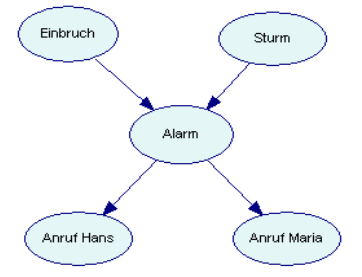
\includegraphics[width=0.5\textwidth]{figures/kap10/bayesian-network.png}
    \caption{Modellierung als Bayes'schen Netze}
    \label{fig:bayesian-net}
\end{figure}

Und das Netzwerk mit den Wahrscheinlichkeitsverteilungen:

\begin{figure}[H]
    \centering
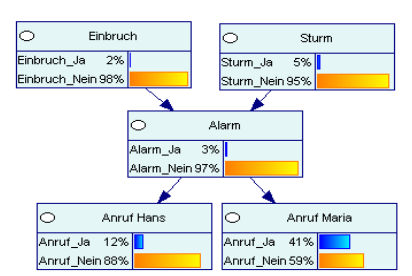
\includegraphics[width=0.6\textwidth]{figures/kap10/bayesian-net-probabilities.png}
    \caption{Modellierung als Bayes'schen Netze}
    \label{fig:bayesian-net-probabilities}
\end{figure}

Wenn sich eine der a-priori Wahrscheinlichkeiten in einem der Knoten �ndert, muss der gesamte Baum neu berechnet werden, um den Baum durch Propagation zu aktualisieren. Wenn zum Beispiel ein Einbruch erkannt wird, dann wird Einbruch\_Ja viel wahrscheinlicher. So kann man mit einem Bayes'schen Netz Inferenzen ziehen.